\documentclass[5p]{elsarticle} % seleccionar: preprint, review, 1p, 3p, 5p



\usepackage{mathtools}
\journal{ }


%to force all images and table in one single section
\usepackage{placeins}
% It is necesary to add \FloatBarrier in the text. 
% After that order, all the floating are shown.

%%%%%%%%%%%%%%%%%%%%%%%
%% Elsevier bibliography styles
%%%%%%%%%%%%%%%%%%%%%%%
%% To change the style, put a % in front of the second line of the current style and
%% remove the % from the second line of the style you would like to use.
%%%%%%%%%%%%%%%%%%%%%%%

%% Numbered
%\bibliographystyle{model1-num-names}

%% Numbered without titles
%\bibliographystyle{model1a-num-names}

%% Harvard
%\bibliographystyle{model2-names.bst}\biboptions{authoryear}

%% Vancouver numbered
%\usepackage{numcompress}\bibliographystyle{model3-num-names}

%% Vancouver name/year
%\usepackage{numcompress}\bibliographystyle{model4-names}\biboptions{authoryear}

%% APA style
%\bibliographystyle{model5-names}\biboptions{authoryear}

%% AMA style
%\usepackage{numcompress}\bibliographystyle{model6-num-names}

%% `Elsevier LaTeX' style
\bibliographystyle{elsarticle-num}

%%%%%%%%%%%%%%%%%%%%%%%
\hyphenation{}
\usepackage{eurosym}
\usepackage{threeparttable} % allow the use of footnote within tables

\usepackage{url}
\usepackage[colorlinks=true, citecolor=blue, linkcolor=blue, filecolor=blue,urlcolor=blue]{hyperref}

%to add the number to the lines
\usepackage{lineno}
\modulolinenumbers[5]

\usepackage{lineno,hyperref}
\modulolinenumbers[1]
\usepackage{amsmath}
\usepackage{siunitx}
\usepackage{eurosym}
\biboptions{numbers,sort&compress}
\usepackage[europeanresistors,americaninductors]{circuitikz}
\usepackage{adjustbox}
\usepackage{xspace}
\usepackage{caption}
\usepackage{booktabs}
\usepackage{tabularx}
\usepackage{threeparttable}
\usepackage{multicol}
\usepackage{float}
\usepackage{graphicx,dblfloatfix}
\usepackage{csvsimple}
%% new commands
\newcommand{\ubar}[1]{\text{\b{$#1$}}}
\newcommand*\OK{\ding{51}}
%\renewcommand*\nompostamble{\end{multicols}}
\newcommand{\specialcell}[2][c]{%
	\begin{tabular}[#1]{@{}l@{}}#2\end{tabular}}
\def\co{CO${}_2$}
\def\el{${}_{\textrm{el}}$}
\def\th{${}_{\textrm{th}}$}


%\renewcommand*{\today}{July, 10 2018}
%\hypersetup{draft} %to avoid problems with hyperref while drafting

\begin{document}

\begin{frontmatter}

\title{The benefits of ambitious short-term targets when decarbonising the coupled electricity and heating energy system in Europe}

%\author[mymainaddress,iClimate]{Marta Victoria\corref{mycorrespondingauthor}}
%\ead{mvp@eng.au.dk}
%\author[mymainaddress]{Kun Zhu}
%\author[kitaddress]{Tom Brown}
%\author[mymainaddress,iClimate]{Gorm B. Andresen}
%\author[mymainaddress,iClimate]{Martin Greiner}
%\cortext[mycorrespondingauthor]{Corresponding author}
%\address[mymainaddress]{Department of Engineering, Aarhus University, Inge Lehmanns Gade 10, 8000 Aarhus, Denmark}
%\address[iClimate]{iCLIMATE Interdisciplinary Centre for Climate Change, Aarhus University}
%\address[kitaddress]{Institute for Automation and Applied Informatics (IAI), Karlsruhe Institute of Technology (KIT), Forschungszentrum 449, 76344, Eggenstein-Leopoldshafen, Germany}



\begin{abstract}



\end{abstract}

\begin{keyword}

%storage, energy system modelling, sector coupling, grid integration of renewables, transmission grid, CO2 emission targets

%\texttt{elsarticle.cls}\sep \LaTeX\sep Elsevier \sep template
%\MSC[2010] 00-01\sep  99-00
\end{keyword}

\end{frontmatter}

%\linenumbers

Achieving a climate-neutral European Union in 2050 \cite{in-depth_2018} requires meeting the in-between milestones. Although carbon emissions will most probably curb by 20\% in 2020, relative to 1990 \cite{EEA_totalGHG}, it is unclear whether this will be the case for the -40\% objective settled for 2030. The national energy plans for the coming decade submitted by member states do not add up the necessary reduction to meet the target \cite{EU-appraisal_2019}. At the same time and led by young people \cite{Warren_2019}, society is claiming for more ambitious climate actions \cite{Rinscheid_2019}. Electricity generation is expected to spearhead the transition spurred by the dramatic cost reduction of wind \cite{Lantz_2012} and solar photovoltaics (PV) \cite{Creutzig_2017, Haegel_2019}. A vast body of literature shows that a power system based on wind, solar, and hydro generation can supply hourly electricity demand in Europe as long as proper balancing is provided 
\cite{Eriksen_2017, Schlachtberger_2017, Gils_2017a, Brown_response}. This can be done reinforcing interconnections among neighbouring countries \cite{Rodriguez_2014} to smooth renewable fluctuations by regional aggregation or through temporal balancing using local storage \cite{Rasmussen_2012, Cebulla_2017}. Moreover, coupling the power system with other sectors such as heating or transport could provide additional flexibilities facilitating the system operation and simultaneously helping to abate emissions in those sectors \cite{Connolly_2016, Brown_2018, Child_2019}. 

CO$_2$ emissions from heating in residential and services sector show a more modest historical reduction trend than electricity generation (Fig. \ref{fig_carbon_budget}). Nordic countries have been particularly successful in reducing carbon emissions from the heating sector by using sector-coupling strategies (Supplementary Note 3). Denmark, where more than half of the households are connected to district heating systems \cite{Gross_2019}, has shifted the fuel used in Central Heat and Power (CHP) units from coal to biomass and urban waste incineration \cite{DEA_2015}. The high penetration of heat pumps in Sweden can be explained by a path-dependence process \cite{Gross_2019} and it is now supported by high CO$_2$ prices \cite{Carbon_pricing_2019} and low electricity taxes. 

Greenfield optimisation of the future European energy system, that is, building the system from scratch, shows that sector-coupling decreases the system cost and reduces the need for extending transmission lines due to the additional local flexibility brought by heating and transport sectors \cite{Brown_2018}. Sector-coupling allows further CO$_2$ reductions before large capacities of storage become necessary, providing more time to develop further storage technologies \cite{Victoria_2019_storage}. Greenfield optimisation is useful to investigate the optimal configuration of the fully-decarbonised system, but it does not provide insights on how to transition towards it. Today's generation fleet and decisions taken in intermediate steps will shape the final configuration. 
Alternative transition paths for the European power system have been analysed using myopic optimisation, without full foresight over the investment horizon \cite{Bogdanov_2019, Plesmann_2017, Gerbaulet_2019, Poncelet_2016}. Myopic optimisation results in higher cumulative system cost than optimising the entire transition period with perfect foresight because the former leads to stranded investments \cite{Gerbaulet_2019, Heuberger_2018}. However, the myopic approach is less sensitive to the assumed discount rate and can capture better short-sighted behaviour of political actors and investors. 

Here, we use a sector-coupled networked model of the European energy system and myopic optimisation in 5-years steps from now to 2050 to investigate the impact of different CO$_2$ restriction paths with the same carbon budget. In every time step, the expansion of generation, storage, and interconnections capacities in every country is allowed  if it results cost effective under the corresponding global emissions constraint. We show that a transition path with more ambitious short-term CO$_2$ targets reduces the cumulative system cost and requires more stable build rates, which are beneficial from the point of view of social acceptance, local industry, and jobs creation. Compared to existing transition paths analyses for the European power system \cite{Plesmann_2017, Gerbaulet_2019, Poncelet_2016}, our research includes the coupling with the heating \textcolor[rgb]{1,0,0}{(and transport)} sector. The use of alternative CO$_2$ reduction paths with constant cumulative emissions is also a novelty of this work. 

Integrated Assessment Models (IAMs) with similar spatial resolution than our model, i.e., one node per country, have also been used to model the sector-coupled decarbonization of Europe \cite{in-depth_2018, JRC-EU-TIMES, Creutzig_2017}. However, IAMs typically use a much lower time resolution, \textit{e.g.} using a few time slices to represent a full year \cite{JRC-EU-TIMES, Loffler_2019, Poncelet_2016, Babrowski_2014} or considering the residual load duration curve \cite{Creutzig_2017, Ueckerdt_2017}. The hourly resolution in our model unveils several effects that are critical to the operation of highly renewable systems, such as the solar and wind non-correlations smoothed by the grid, the role of long-term storage, and the system operation during cold spells, \textsl{i.e.} a cold week with low wind and solar generation . By using an open model, we ensure transparency and reproducibility of the results in a  discipline with high policy relevance such as it is energy modelling \cite{Pfenninger_2017, Pfenninger_2018}. 

\paragraph{\textbf{Carbon budget for electricity and heating in Europe}} \

A remaining global carbon budget of 800 Gigatons (Gt) of CO$_2$ can be emitted from 2017 onwards to limit the anthropogenic warming to 2$^{\circ}$C relative to preindustrial period with a probability of greater than 66\% \cite{Figueres_2017, blog_budget}. Different sharing principles can be used to split the global carbon budget into regions and countries \cite{Raupach_2014}. We consider an equal per-capita distribution that translates into a quota of 48 GtCO$_2$ for Europe. Since the historical quota has been much higher this implies that Europe must be more ambitious than other regions. Assuming that sectoral distribution of emissions within Europe remains at present values, the carbon budget for the generation of electricity and provision of heating in the residential and services sector accounts for approximately 21 GtCO$_2$, \cite{UNFCCC_inventory} and Supplementary Note 1.

\begin{figure}[!h]
\centering
	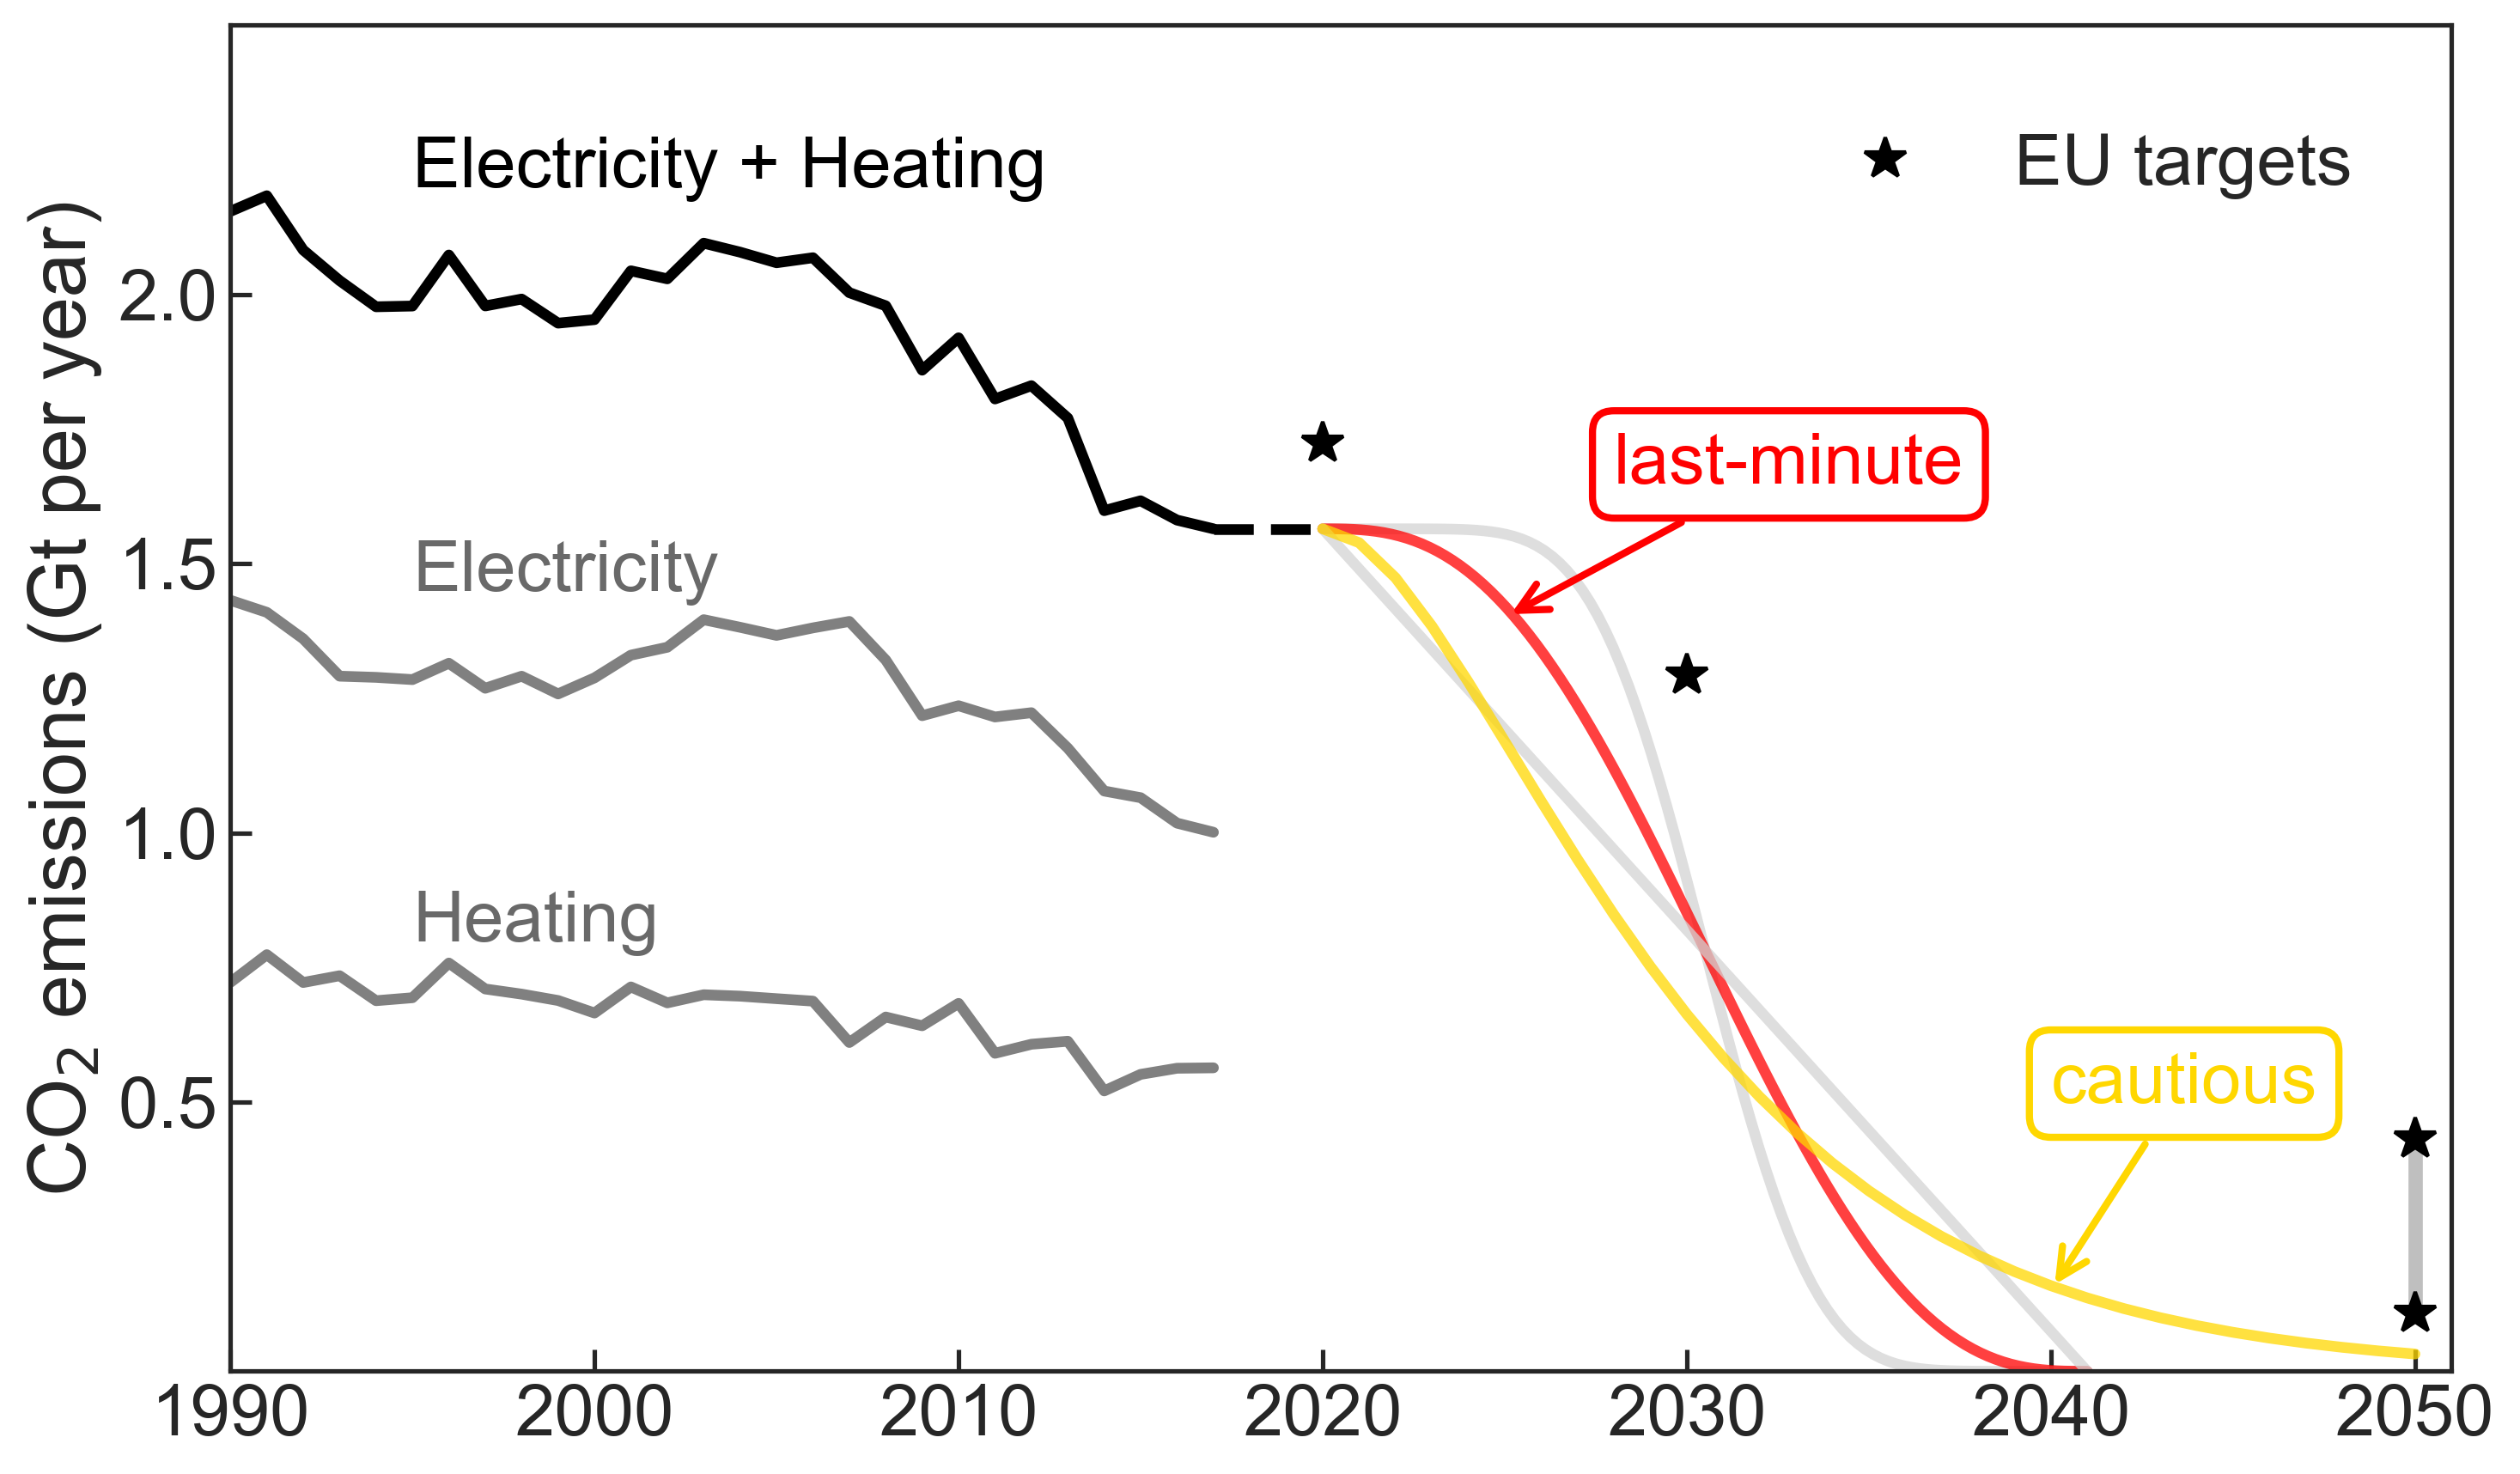
\includegraphics[width=\columnwidth]{figures/carbon_budget.png}
\caption{Historical CO$_2$ emissions from the European power system and heating supply in the residential and services sectors \cite{UNFCCC_inventory}. The various future transition paths shown in the figure have the same cumulative CO$_2$ emissions, which correspond to the remaining 21 Gt CO$_2$ budget to avoid human-induced warming above 2$^{\circ}$C with a probability of greater than 66\%, assuming current sectoral distribution for Europe, and equity sharing principle among regions. The stars indicate committed EU reduction targets.} \label{fig_carbon_budget} 
\end{figure}

\paragraph{\textbf{Stranded assets}} \

The two alternative transition paths arrive at a similar system configuration in 2050. 
Due to their high cost, some of are not selected until the final years, in which heavily restricted CO$_2$, disallows the use of gas and they are necessary to balance renewable generation. This is the case for large storage energy capacities, such as electric batteries and H$_2$ storage, and methanation. Cumulative cost for cautious path represents 9421 billion euros (B\EUR), while last-minute path accounts for 9694 B\EUR. Gas power plants represent the main stranded assets causing the higher cost of last-minute path. The lower CO$_2$ emissions restriction in 2030 and earlier allow the installation of such plants. However, the drastic emissions allowance in subsequent years, avoids the operation of gas power plants. The Europe-averaged utilisation factors shown in Fig. \ref{fig_utilisation_factors} are close to zero from 2040 onwards for the gas units in the last-minute path. For both transition paths, even in the initial years the utilisation factor of gas is below 30\%. This is a consequence of the role that gas units play as backup technology securing electricity and heat supply when there is a significant deficit of renewable generation, but it is also a consequence of the large capacity of gas recently installed in Europe. The pyramid age of existing electricity generation technologies in Europe, Fig. 4 in Supplementary Materials, unveils that most of the `younger' power plants use gas. Since most of the gas capacity in Europe was installed less than 25 years ago, part of this capacity represent a stranded asset during the initial years for both transition paths. Although, infrautilisation of existing generation capacity might be seen as an unnecessary contribution to higher cost of energy it must be remarked that the early retirement of electricity infrastructure has been identified as one of the most cost-effective actions to reduce committed emissions and enable a 2$^{\circ}$C-compatible future evolution of global emissions \cite{Tong_2019}.

\begin{figure*}[!h]
\centering
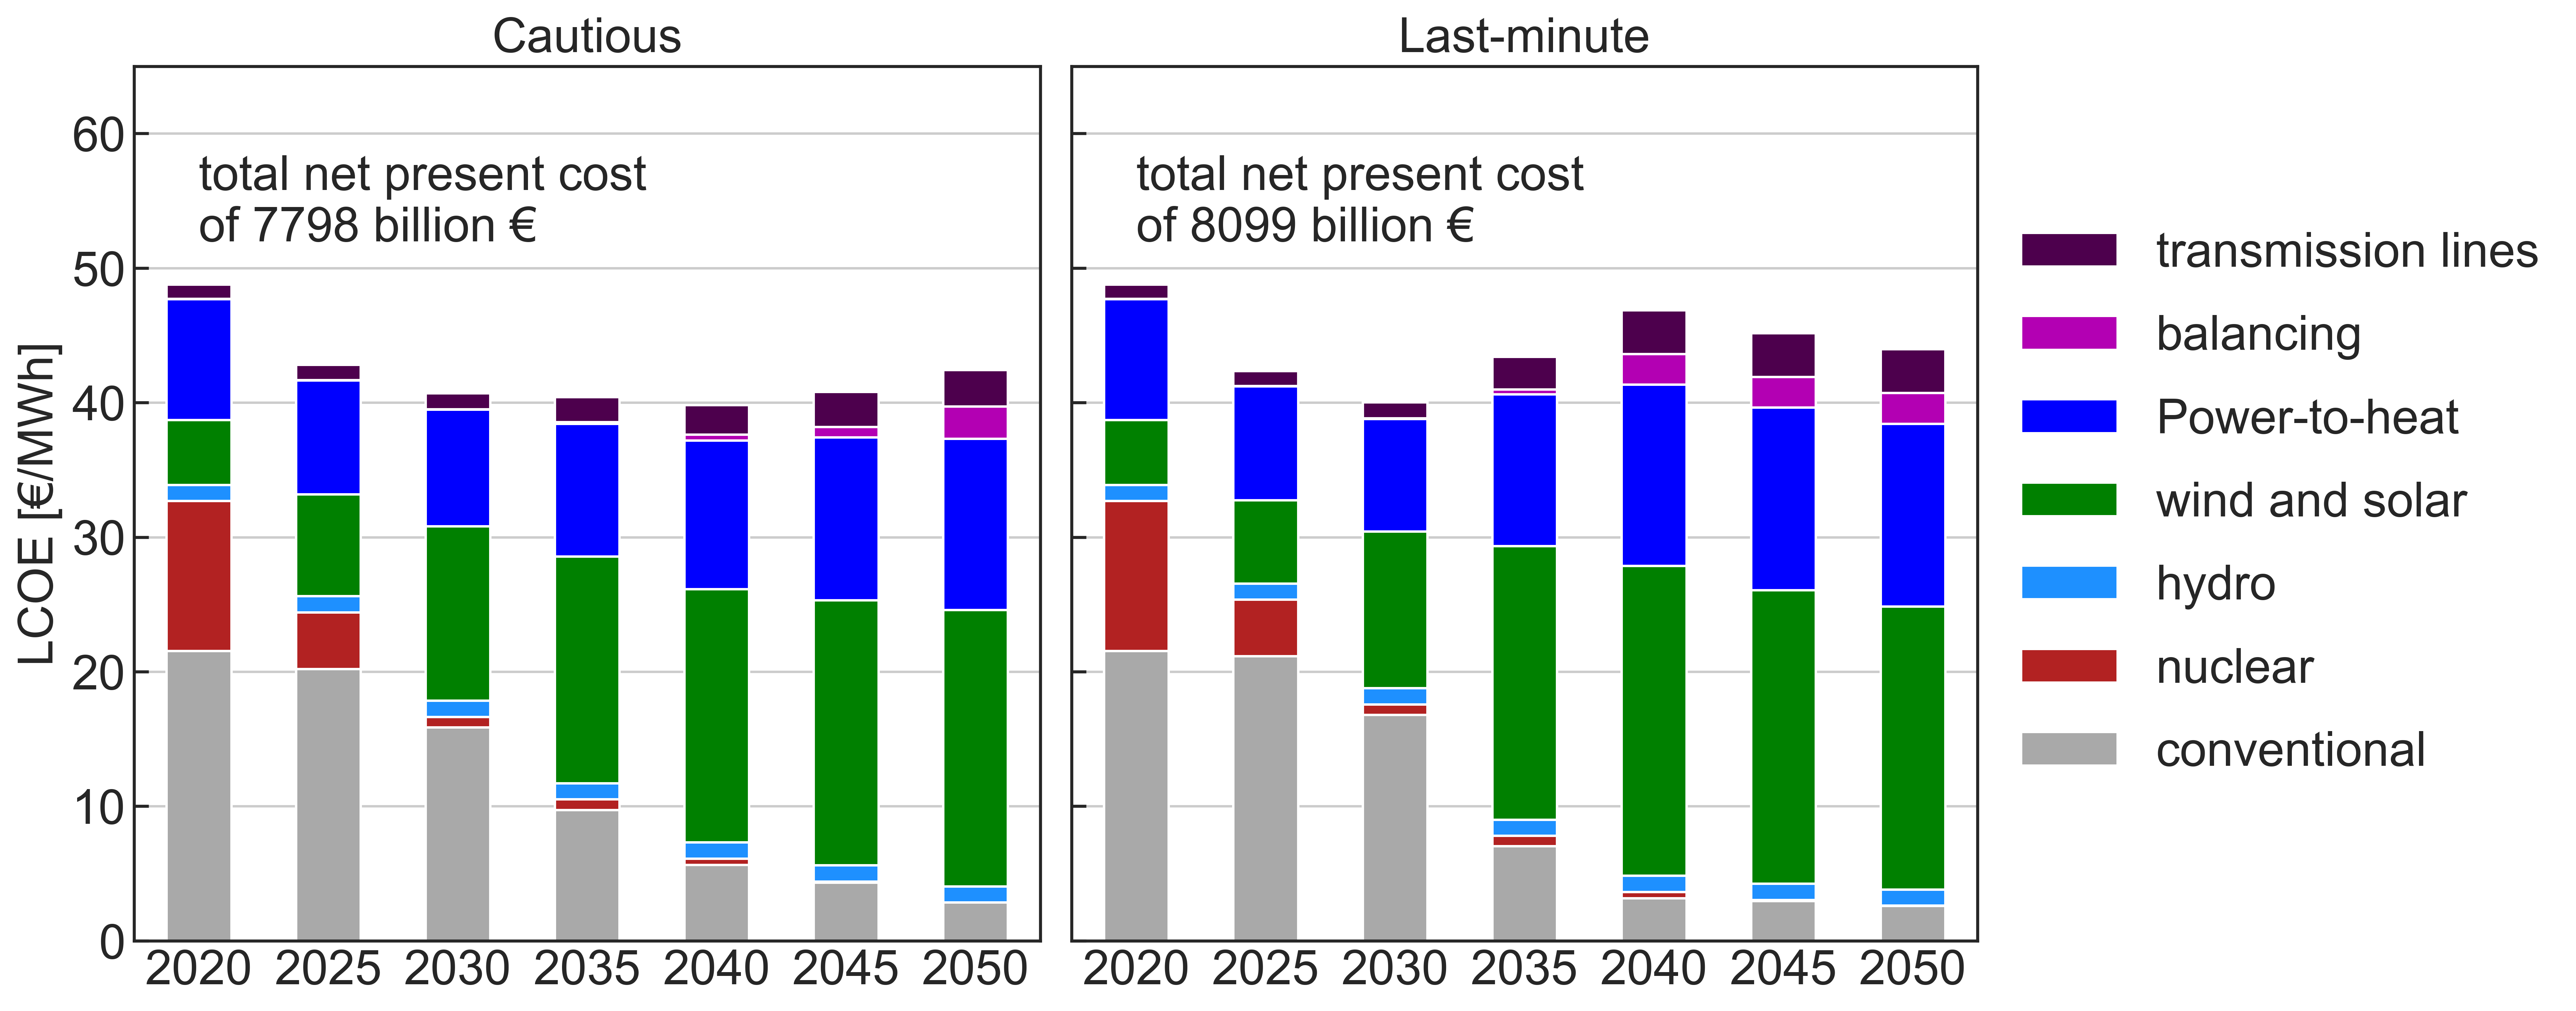
\includegraphics[width=12cm]{figures/LCOE_Base.png}
\caption{Levelized Cost of Energy (LCOE) for the European electricity and heating system throughout transition paths cautious and last-minute shown in Fig. \ref{fig_carbon_budget}. Conventional includes costs associated with coal, lignite, and gas power plants producing electricity as well as gas consumed in gas boilers and CPH units. Power-to-heat category includes costs associated with heat pumps and heat resistors. } \label{fig_system_cost} 
\end{figure*}

\begin{figure}[!h]
\centering
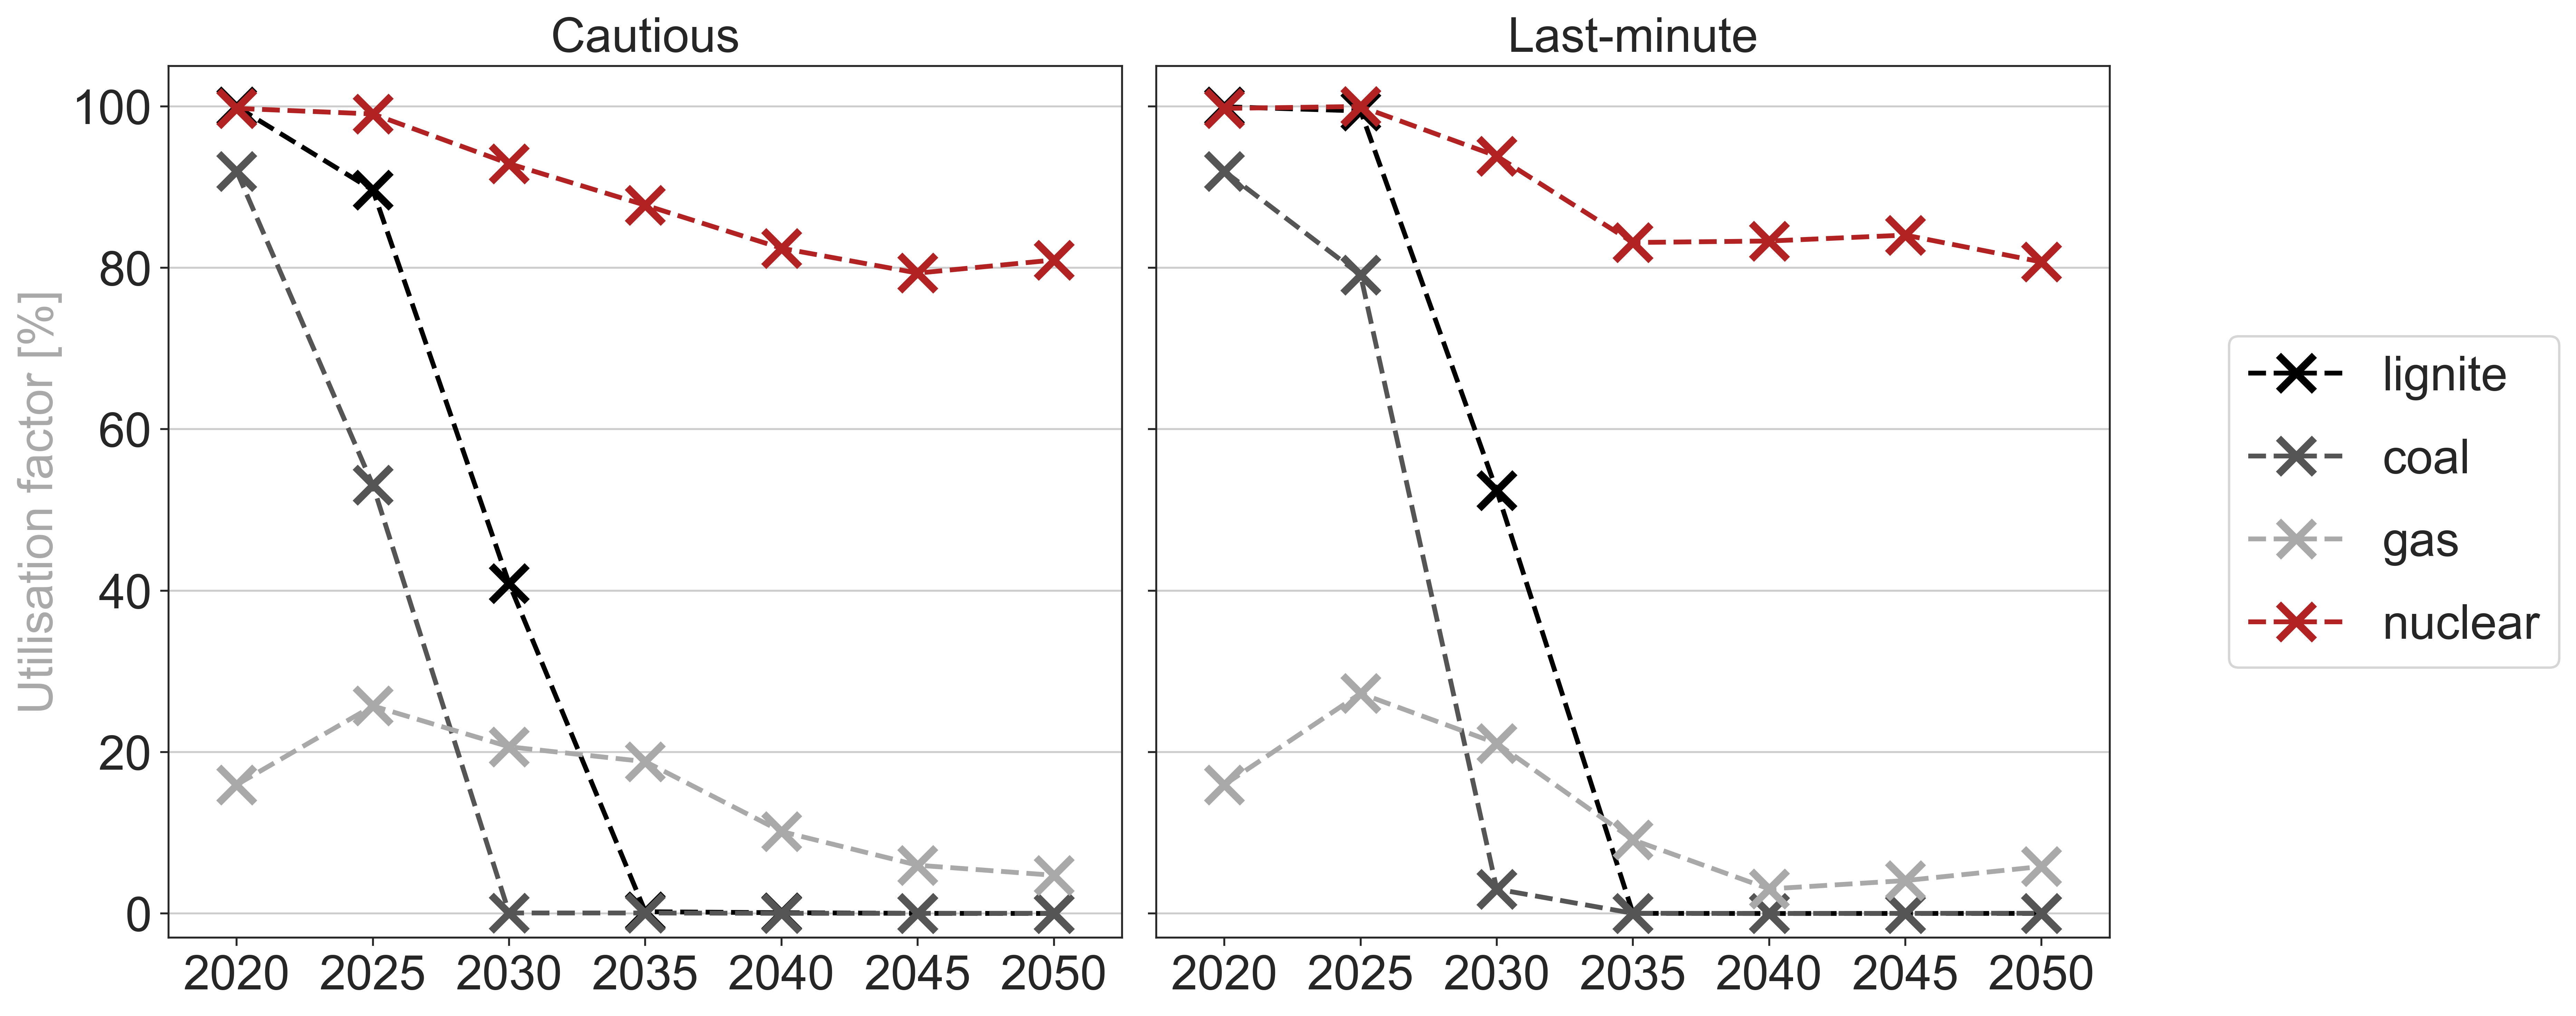
\includegraphics[width=\columnwidth]{figures/utilisation_factors_Base.png}
\caption{Utilisation factors for lignite, coal, gas, and nuclear power plants throughout transition paths cautious and last-minute shown in Fig. \ref{fig_carbon_budget}. The figure also depicts the wind and solar curtailment, as percentage of energy generated by those technologies. } \label{fig_utilisation_factors} 
\end{figure}


\paragraph{\textbf{Build rates and feasibility of transition paths}} \

During the past decade, several European countries have shown sudden increments in the annual build rate for solar PV, followed by equivalent decrements one or two years later. Italy, Germany, Spain, and UK show clear peaks (see Supplementary Note 5)  due to the combination of a fast cost decrease of the technology and unstable regulatory frameworks whose details are country-specific. These peaks are lethal for local businesses. The sudden shrinkage of annual build capacity results into companies bankruptcy and job loss. Fig. \ref{fig_build_rates}  shows the build rates for several technologies throughout the cautious and last-minute paths. The former requires a smoother evolution of build rates which could better accommodate the cultural, political, and social aspects of the transition \cite{Geels_2017}. Although none of the build rates required in the last-minute path is technological infeasible, the cautious path is more compatible to the inertias in the transition such as required time to modify regulatory frameworks or to educate the necessary labour force. 

\begin{figure}[!h]
\centering
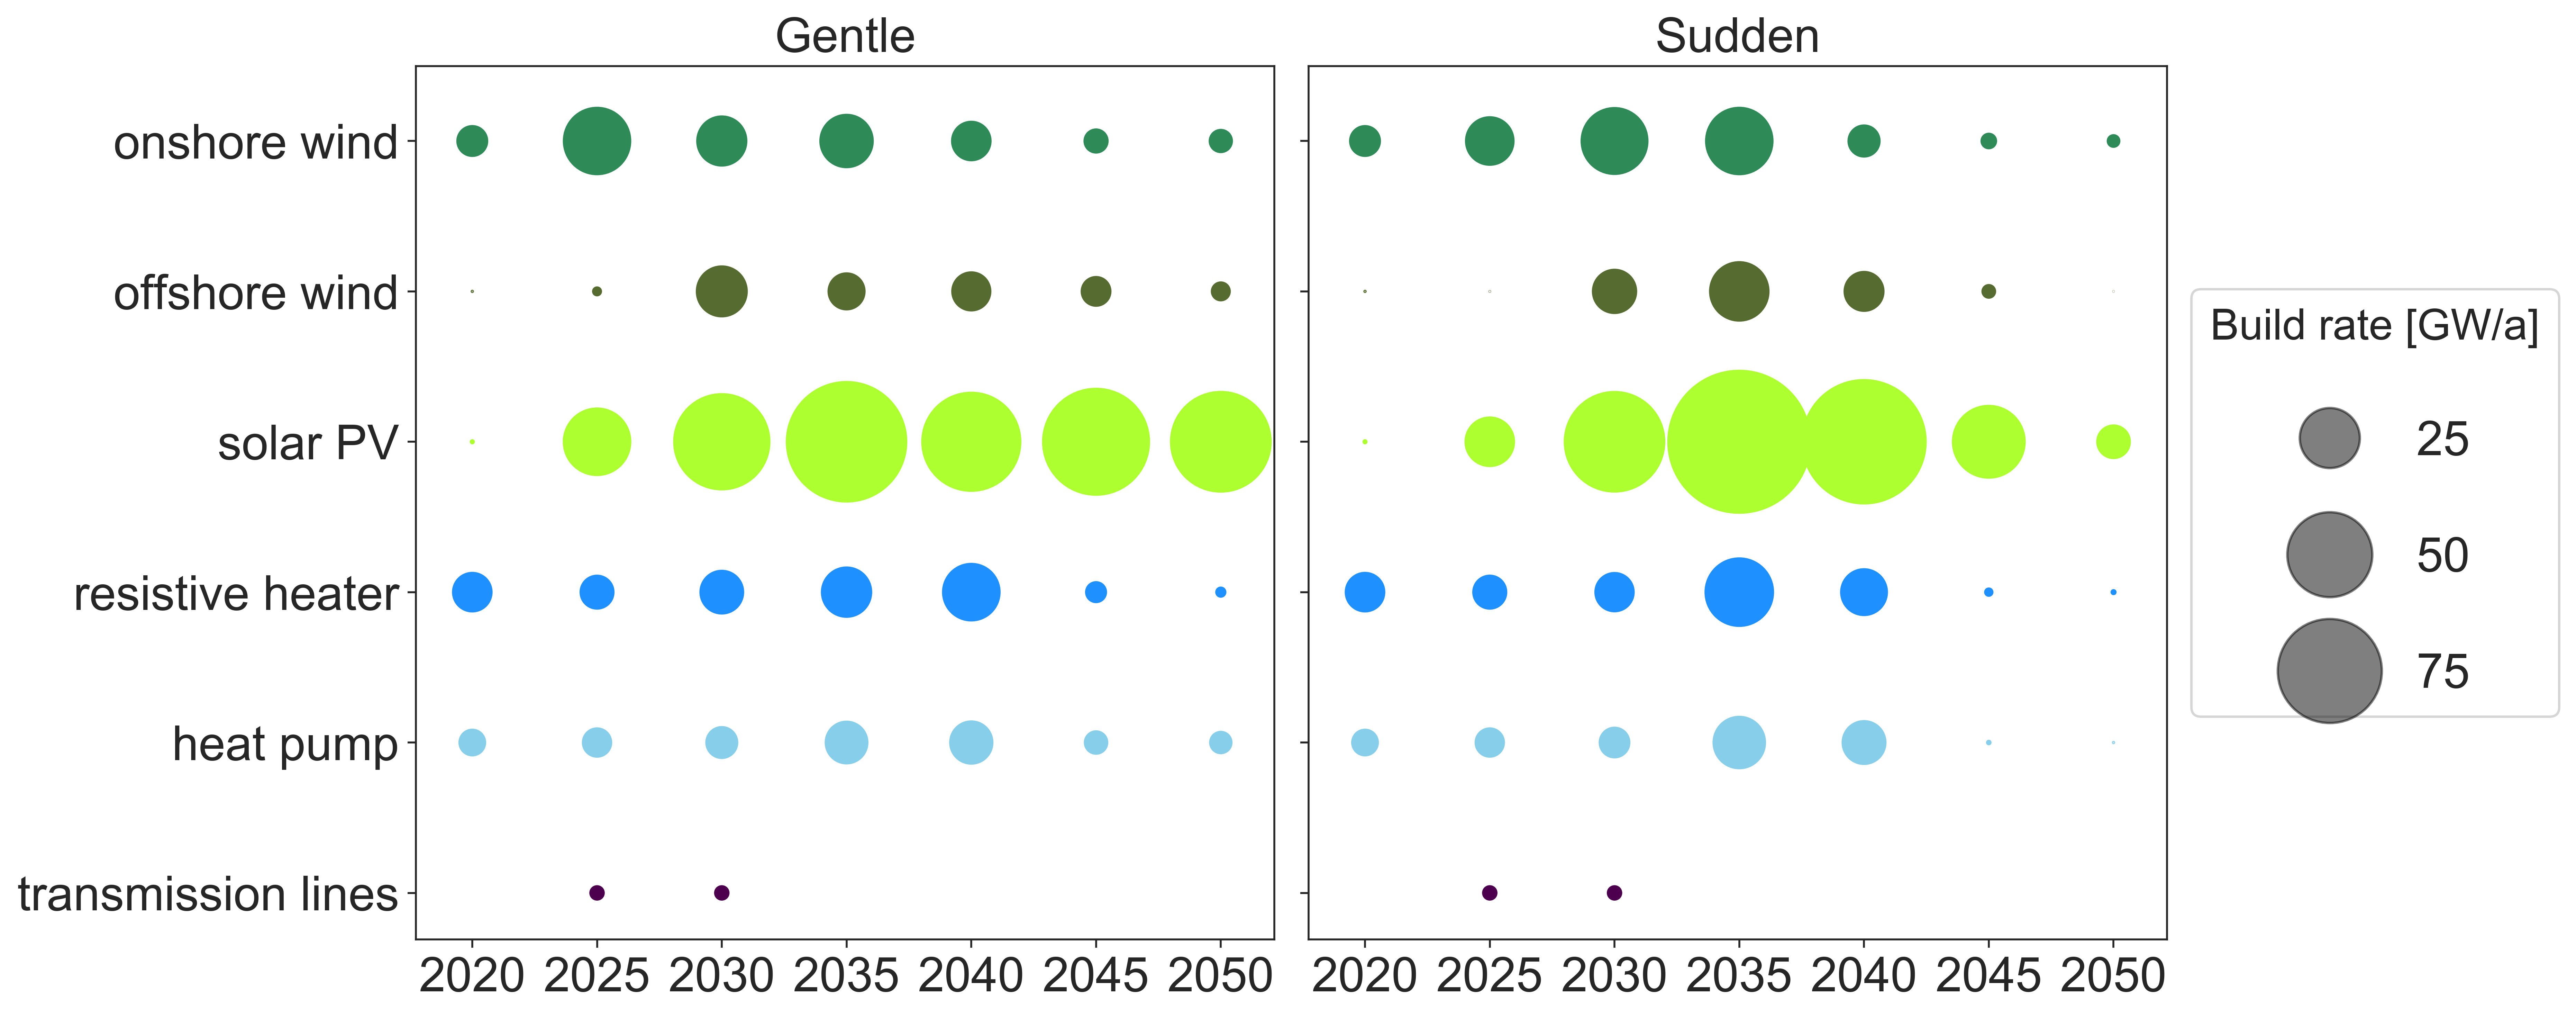
\includegraphics[width=\columnwidth]{figures/build_rates_Base.png}
\caption{Annual build rates for different technologies throughout transition paths cautious and last-minute shown in Fig. \ref{fig_carbon_budget}. \textcolor[rgb]{1,0,0}{TODO: We are considering making a new Figure combining these results with the historical installation rates shown in Fig. 4 in the Supplementary Materials.} } \label{fig_build_rates} 
\end{figure}


\paragraph{\textbf{Balancing renewable generation}} \

\textcolor[rgb]{1,0,0}{TODO: Write paragraph discussing the country-specific mix of primary energy and reference previous results regarding balancing. Discuss also the difference between the 2050 results with the cautious path and using greenfield optimization, using the spatial plot figure in the Supplementary Materials.}

\begin{figure*}[!h]
\centering
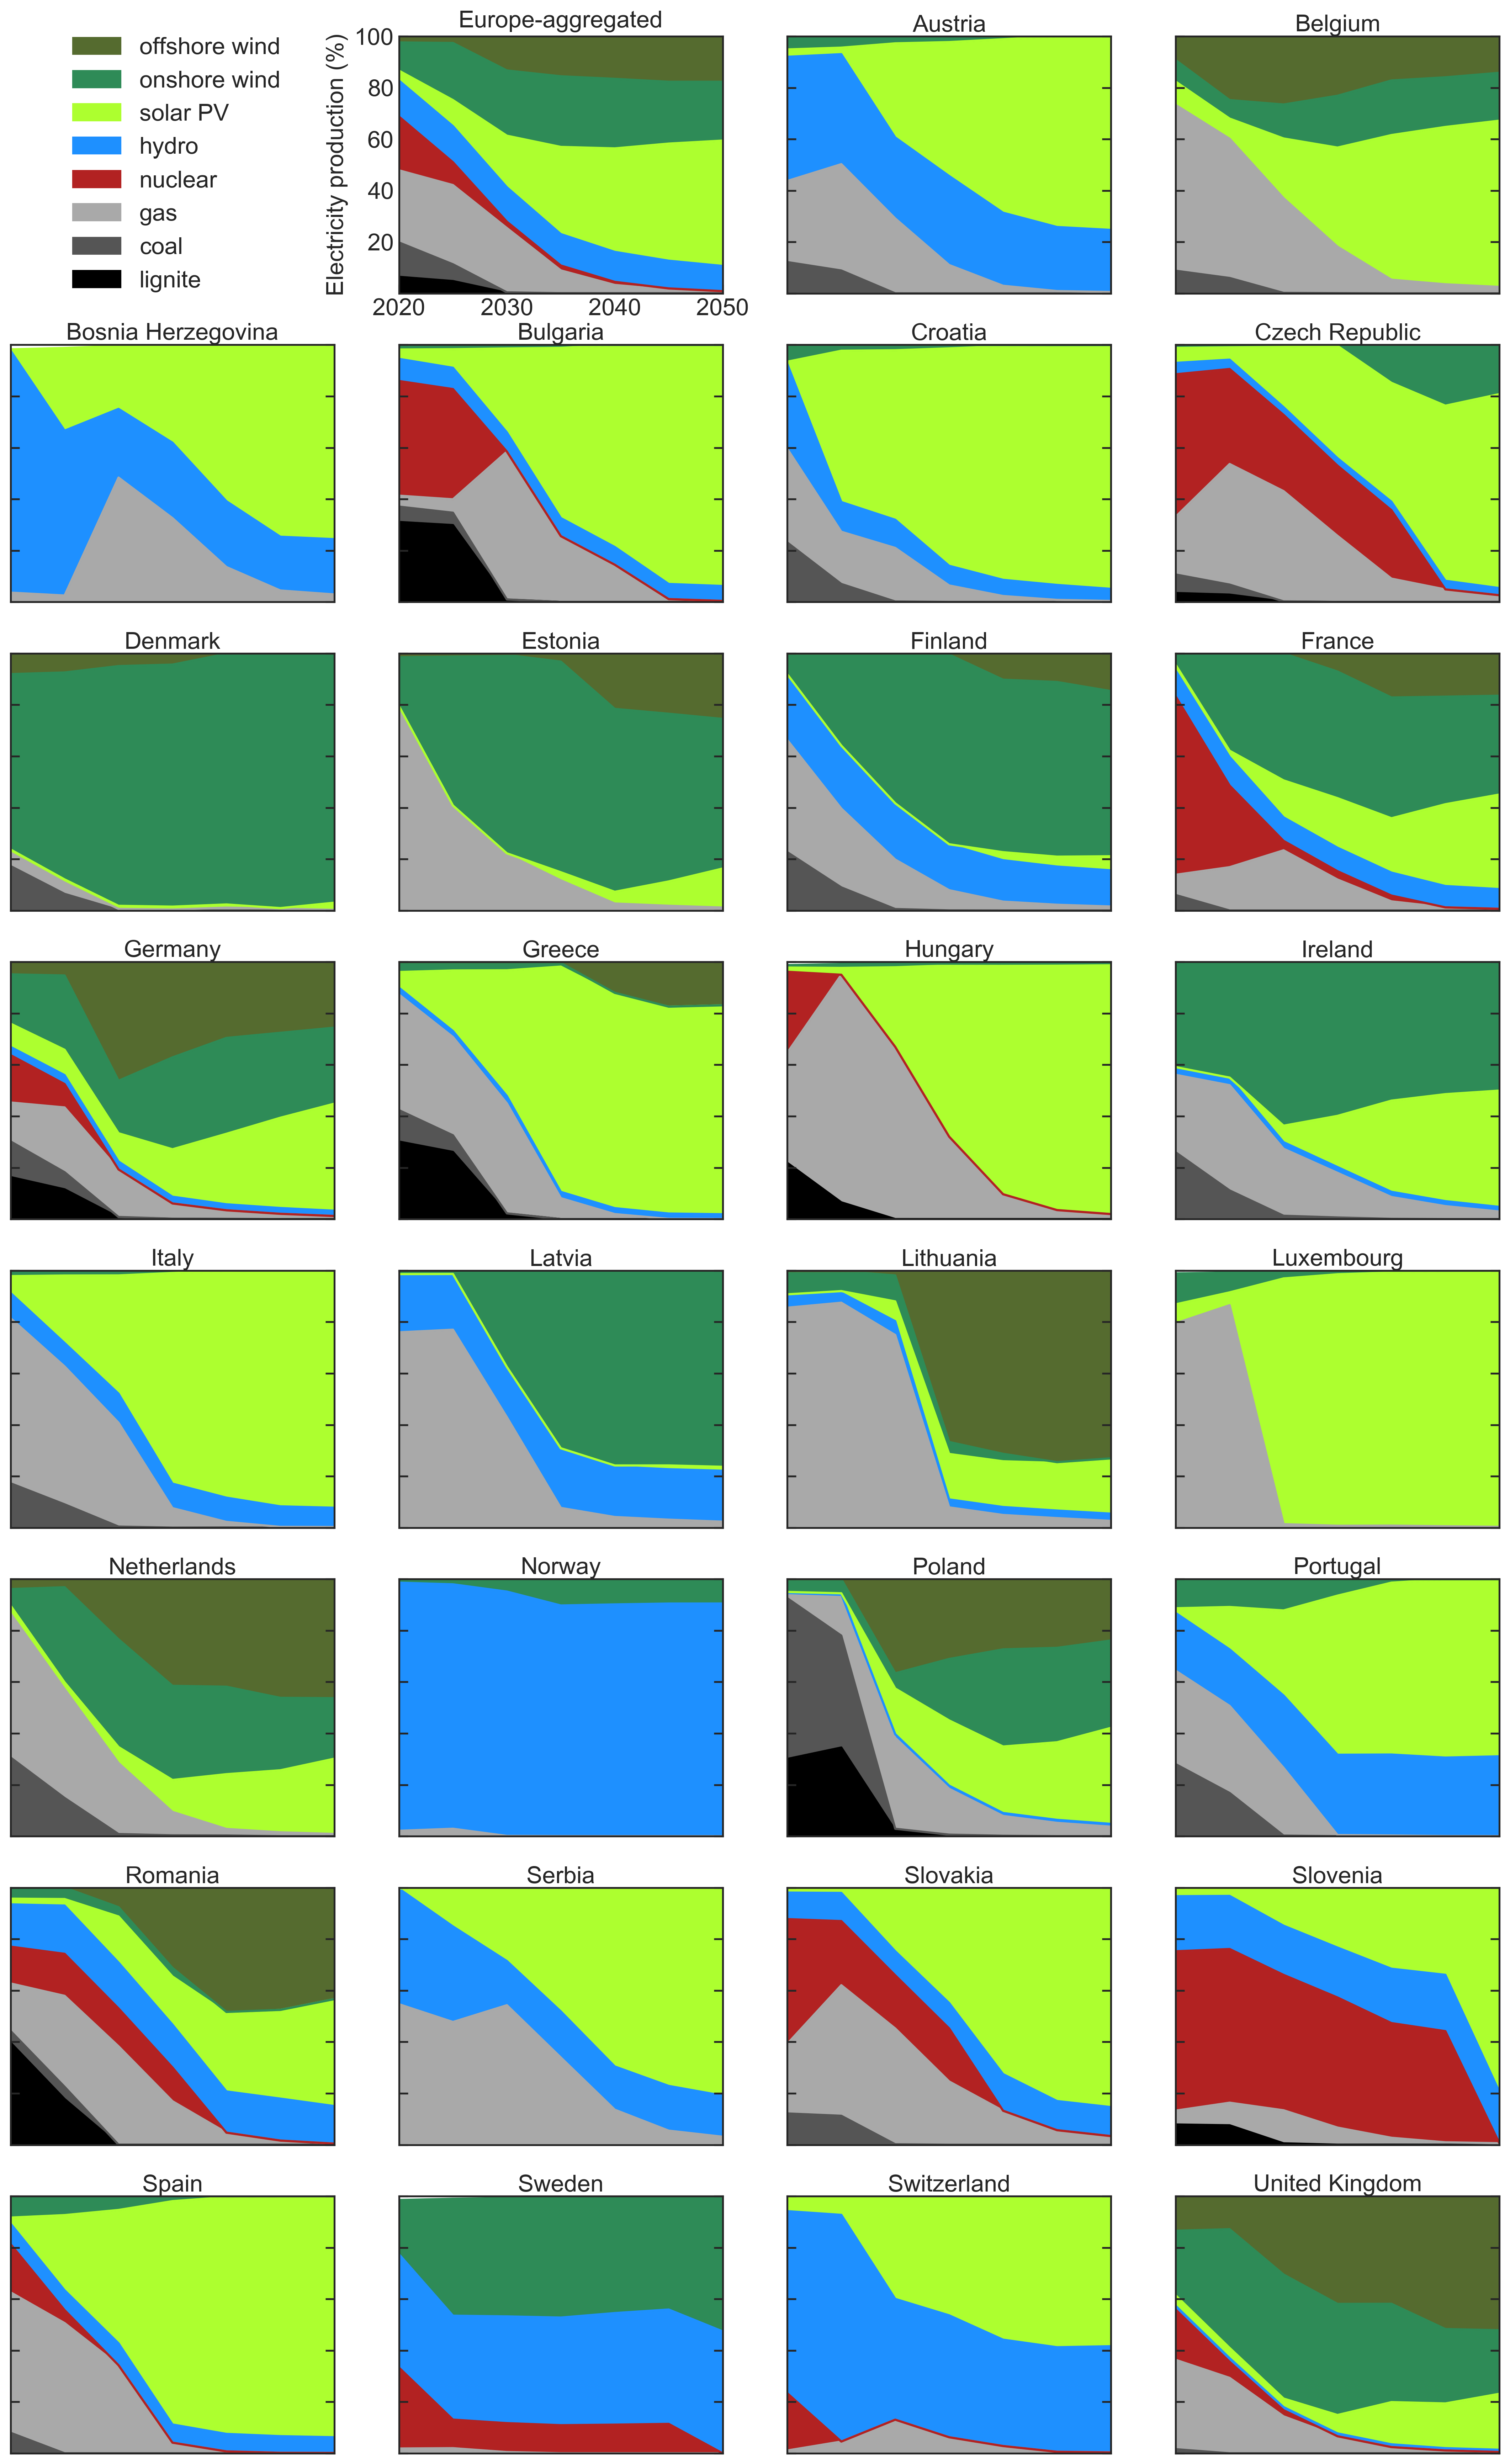
\includegraphics[width=14cm]{figures/electricity_production_Base_go.png}
\caption{Evolution of electricity generation mix in every country for the transition path cautious.} \label{fig_primary_energy} 
\end{figure*}

\paragraph{\textbf{Policy incentives are needed}} \

\textcolor[rgb]{1,0,0}{TODO: Write paragraph discussing evolution of CO$_2$ price. Include caveat due to not modelling biomass. Add comment on possible alternative to setting CO2 price such as economic aids for certain technologies. We use CO$_2$ price here, other measures can also be efficient. }

\begin{figure}[!h]
\centering
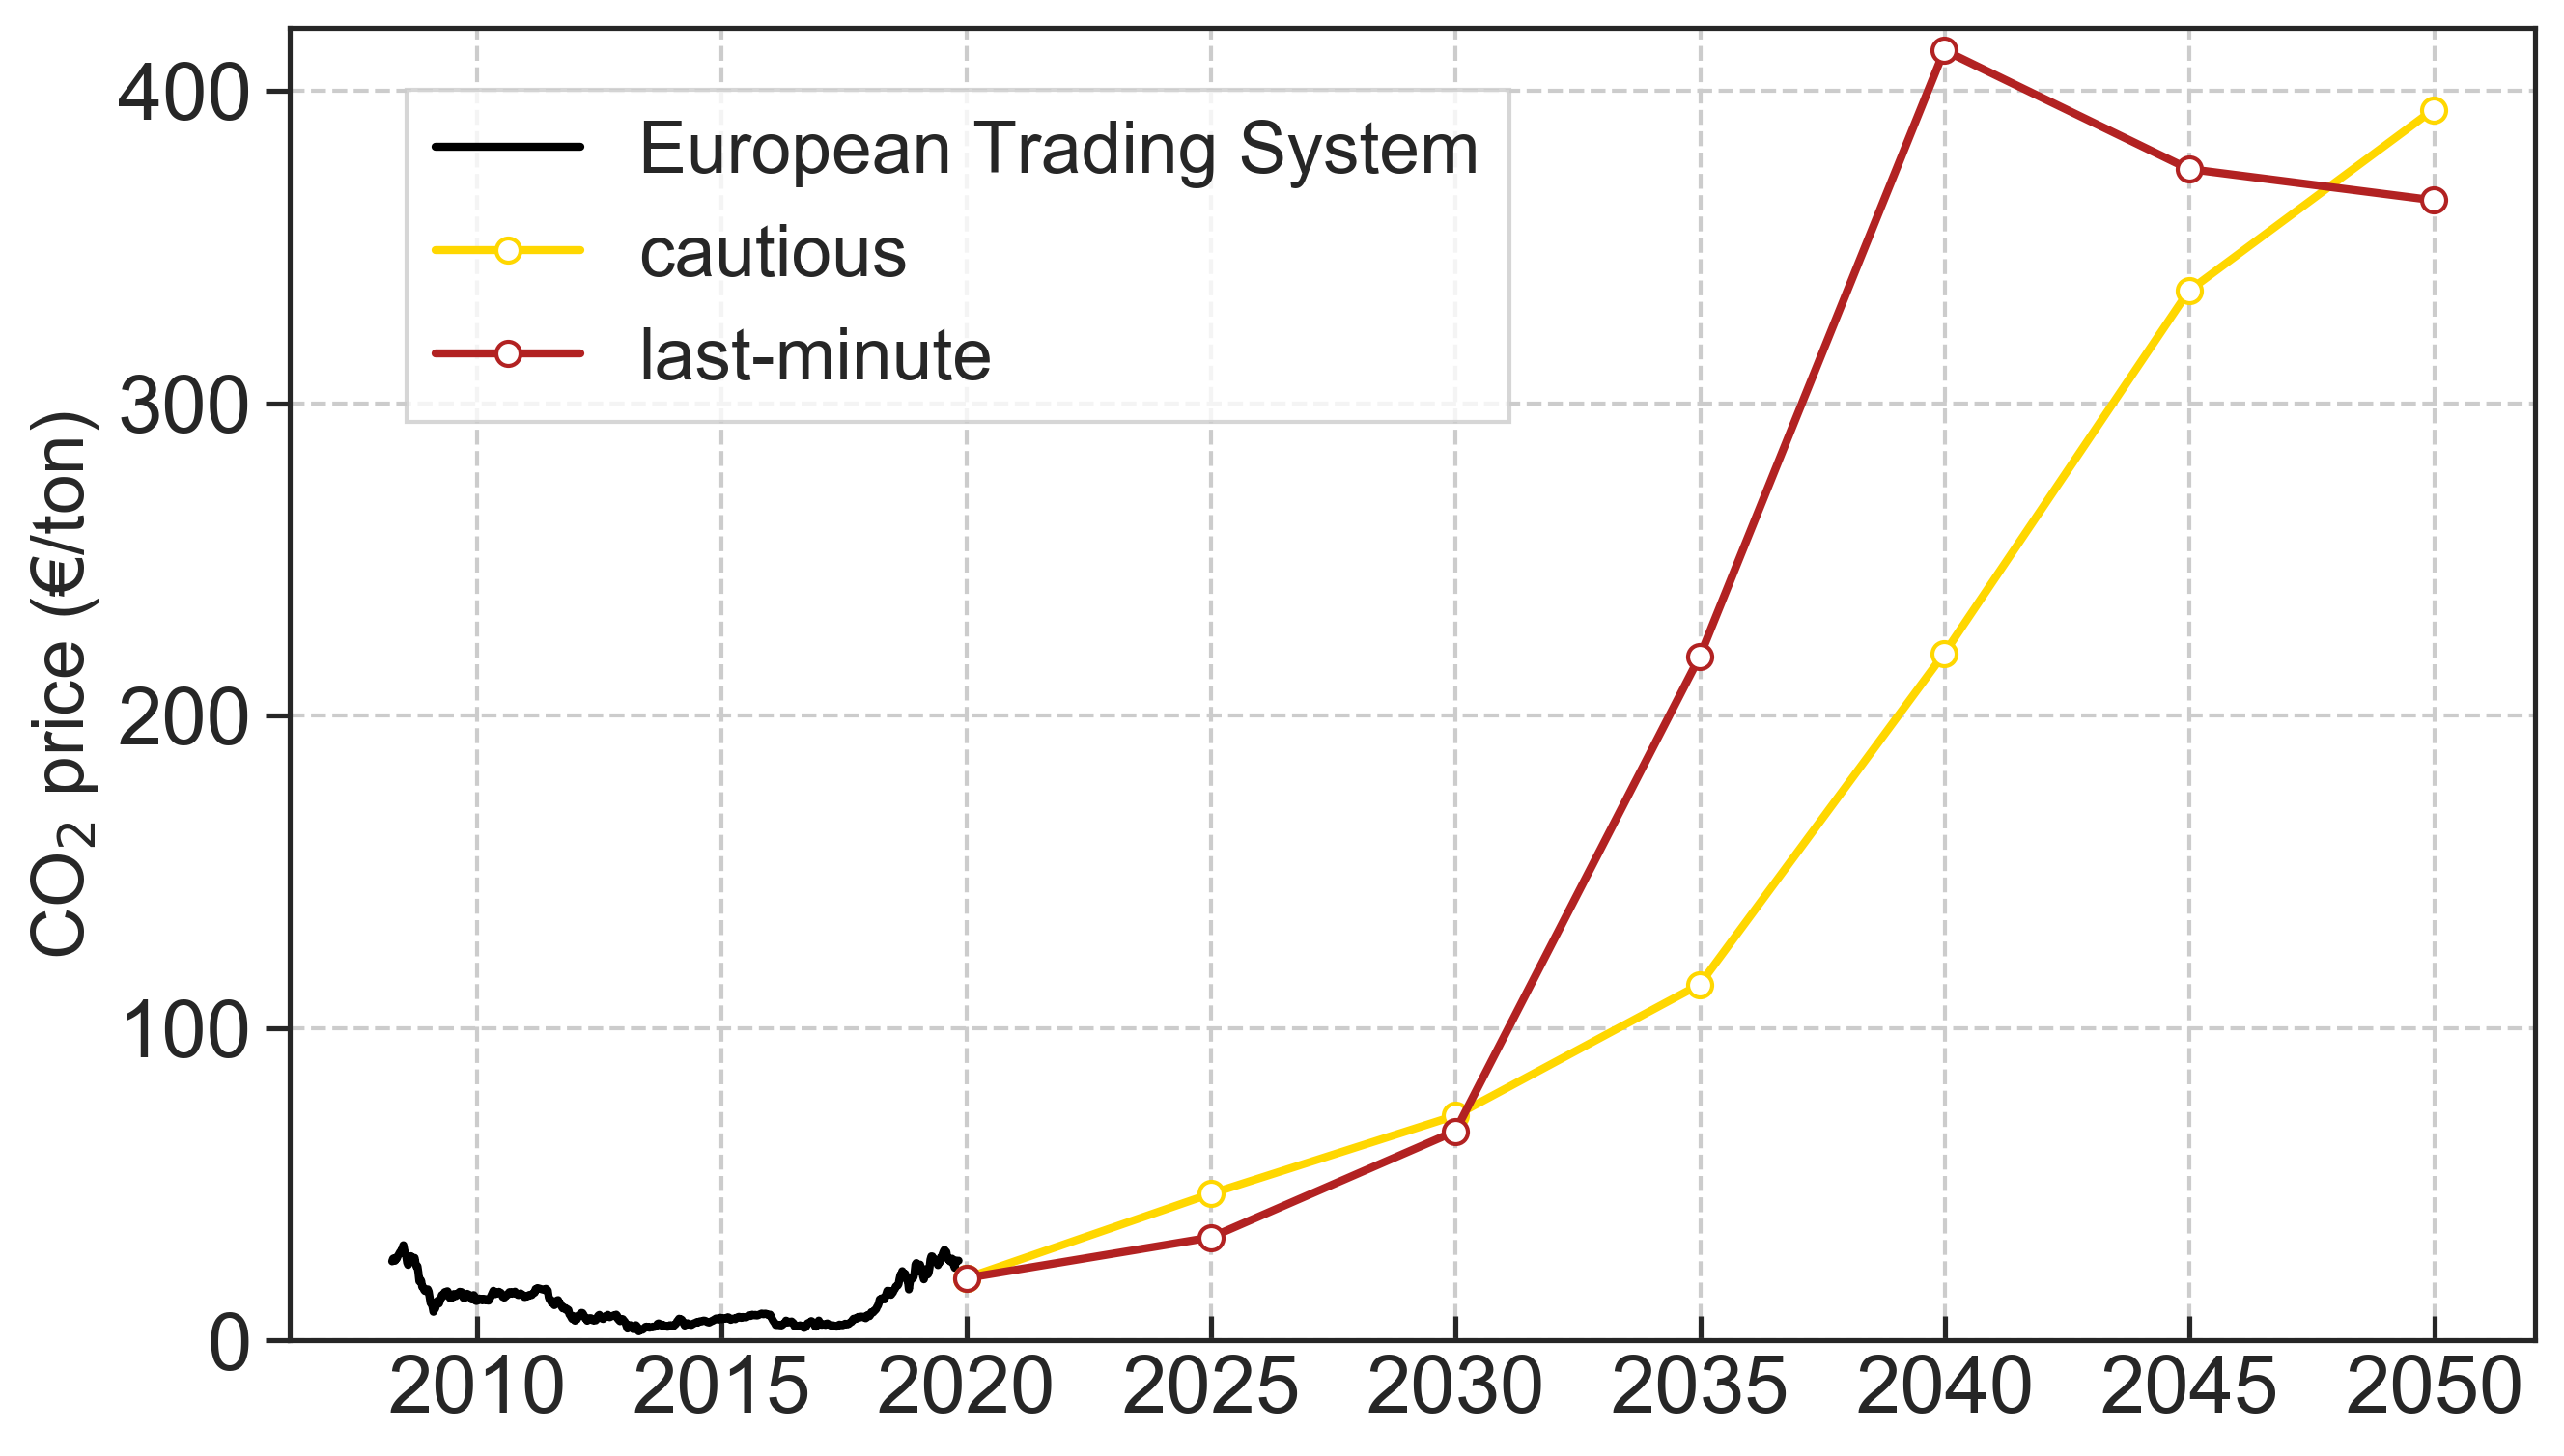
\includegraphics[width=\columnwidth]{figures/co2_price.png}
\caption{Historical evolution of CO$_2$ price in the European Trading System \cite{ETS} and required CO$_2$ price obtained from the model throughout transition paths cautious and last-minute shown in Fig. \ref{fig_carbon_budget}} \label{fig_co2price} 
\end{figure}

\paragraph{\textbf{Transitioning without grid expansion}} \

\textcolor[rgb]{1,0,0}{TODO: Write paragraph discussing the different results
obtained when the expansion of transmission lines after 2030 is not allowed. }

\paragraph{\textbf{Early action allows room for decision-making later}} \

\textcolor[rgb]{1,0,0}{TODO: Run cautious path banning the use of coal and lignite after 2025/2030 and write paragraph discussing the results}


\paragraph{\textbf{The challenging decarbonisation of the heating sector}} \

\textcolor[rgb]{1,0,0}{TODO: Run cautious path banning new district heating and write paragraph discussing the results}

\paragraph{\textbf{Impact of building retrofitting}} \

\textcolor[rgb]{1,0,0}{TODO: Run cautious path including path for reduction of heating demand, e.g. 3\% per year and write paragraph discussing the results}

\paragraph{\textbf{Coupling the transport sector}} \

\textcolor[rgb]{1,0,0}{TODO: Run cautious path including path representing the electrification of the transport sector and write paragraph discussing the results.}

\paragraph{\textbf{Heterogeneity among European countries}} \

\textcolor[rgb]{1,0,0}{TODO: Discuss final system configuration obtained as a result of the path vs. greenfield optimization in 2050.}

%\begin{footnotesize}
\section{Methods}

The system configuration is optimised by minimising annualised system cost in every time step (one every 5 years), under the global CO$_2$ emissions cap imposed by the transition path under analysis (Fig. \ref{fig_carbon_budget}). This can be considered a myopic approach since the optimisation has no information about the future. The cumulative CO$_2$ emissions for all the different transition paths is equal to a carbon budget of 21 GtCO$_2$. In every time step, generation, storage, and transmission capacities in every country are optimised assuming perfect competition and long-term market equilibrium. Besides the global CO$_2$ emission cap, other constraints such as the demand-supply balance in every node, and the maximum power flowing through the links are imposed to ensure the feasibility of the solution, see Supplementary Note 6. \

We use a one-node-per-country network, including 30 countries corresponding to the 28 European Union member states as of 2018 excluding Malta and Cyprus but including Norway, Switzerland, Bosnia-Herzegovina, and Serbia (Fig. \textcolor[rgb]{1,0,0}{X} in the Supplementary Notes). Countries are connected by High Voltage Direct Current (HVDC) links whose capacities can be expanded if it is cost-effective. In the power sector, electricity can be supplied by onshore and offshore wind, solar photovoltaics (PV), hydroelectricity, Open Cycle Gas Turbines (OCGT), Combined Cycle Gas Turbines (CCGT), Coal, Lignite, and Nuclear power plants, and Combined Heat and Power (CHP) units using gas. Electricity can be stored using Pumped Hydro Storage (PHS), static electric batteries, and hydrogen storage. Hydrogen is produced via electrolysers and converted back into electricity using fuel cells. Methane can be produced by combining Direct Air Captured (DAC) CO$_2$ and electrolysed-H$_2$ in the Sabatier reaction.  
%Historical time series from 2015 are used to represent electricity demand. Future demands increments in our model are captured via heat demands or transport demand when included.  
Heating demand is split into urban heating, corresponding to regions whose population density allows centralised solution, and rural heating where only individual solutions are allowed. Heating can be supplied via central heat pumps, heat resistors, gas boilers, solar collectors, and CHP units for urban regions, while only individual heat pumps, electric boilers, and gas boilers can be used in rural areas. Centralised and individual thermal energy storage can also be installed. A detailed description of all the sector is provided in the Supplementary Note 7. \

Costs assumed for the different technologies depend on time (Supplementary Note 8) but not on the cumulative installed capacity since we assume that they will be influenced by the forecast global installation rates and learning curves. The financial discount rate applied to annualise costs is equal to 7\% for every technology and country. Although it can be strongly impacted by the maturity of a technology and the rating of a country \cite{Egli_2019}, we assumed European countries to be similar enough to use a constant discount rate. The already installed capacities, \textit{i.e.} existing capacities in 2020 or capacities installed in a previous year whose life time has not concluded, are exogenously included in the model. For every time step, the total system cost includes two components. First, the costs of newly installed assets, which exactly recover their investment by market revenues. Second, the stranded costs for the exogenously fixed capacities. They are determined as the difference between the annualised costs and the revenues that those assets get from the market.  To estimate the cumulative cost of every transition path, the annualised cost for all year are added assuming a social discount rate of 2\%. This rate represents the value at which we, as European society, discount investments in far-future years when comparing them with present investments. We have selected a social discount rate of 2\%, which is similar to the inflation rate in the European Union, that averaged 2.4\% in the past 20 years. It is worth remarking that the cumulative cost remains lower for the last-minute path provided that discount rates lower than 11\% are assumed. The CO$_2$ price is not an input to the model, but a result that is obtained via the Lagrange/Karush-Kuhn-Tucker multiplier associated with the global CO$_2$ constrain. 
%\end{footnotesize}

\section{Data availability and code availability}

\section{References}
\bibliography{bib_transition}

\end{document}